

\chapter{Grundlagen zu Neo4j} % Main chapter title

\label{Kaptiel 2} % Change X to a consecutive number; for referencing this chapter elsewhere, use \ref{ChapterX}

%----------------------------------------------------------------------------------------
%	SECTION 1
%----------------------------------------------------------------------------------------
\section{Graph als Datenstruktur}
Ein Graph ist eine abstrakte Datenstruktur, welche aus der Mathematik stammt \parencite{vicknair2010comparison}. Graphen werden als ein geordnetes Triple (V(G), E(G), $\psi_G$) aufgefasst, für GBDs sind V(G) und E(G) endliche Mengen. V(G) ist eine nicht leere Menge von Knoten, auch Punkte genannt. E(G) ist eine Menge der Kanten. Die Funktion $\psi$ weist jeder Kante ein Tupel aus Knoten, so stellt $\psi_G (e) = (v_1 v_2)$ eine Verbindung der Knoten $v_1$ und $v_2$ durch die Kante $e$ dar. Wenn $\psi$ ein geordnetes Tupel von Knoten verwendet und die Reihenfolge somit relevant ist, besitzt die Kante  eine  Richtung und der Graph wird als gerichtet bezeichnet, bei einem ungeordneten Paar wird von einem ungerichteten Graph gesprochen. Wenn die Kanten Gewichte oder Kosten zur Traversierung besitzen, wird der Graph als gewichtet bezeichnet und ohne Gewichte als ungewichtet \parencite{bondy1976graph}.

\section{Temporale Datenbanken}
Eine temporale Datenbank besitzt die Fähigkeit, alle Daten in Abhängigkeit von einer zeitlichen Einheit zu speichern \parencite{campos2016towards}. Jede Relation und Entität kann ein Datum besitzen, zu welchem der Eintrag gültig ist. Zu jedem  Zeitpunkt, der nicht diesem Datum entspricht, ist es nicht garantiert, dass der betrachtete Eintrag in der Datenbank gültig ist. Wenn eine Person zu einem genannten Zeitpunkt bei einer Firma angestellt ist und kann zu einem Zeitpunkt, der nach dem genannten Zeitpunkt folgt, keine garantierte Aussage getroffen werden, ob die Person noch bei der Firma angestellt ist. \newline
Die Entitäten und Relationen können auch Attribute von einem zeitlichen Datentypen besitzen, welches eine bestimmte Eigenschaft beschreibt und nichts über die Gültigkeit aussagt\parencite{khurana2012introduction}.  
%-----------------------------------
%	SUBSECTION 1
%-----------------------------------
\section{Überblick zu Neo4j}
Neo4j ist eine temporale Graphdatenbank, welche in Java implementiert wurde \parencite{vukotic2015neo4j}. Als grundlegende Datenstruktur wird ein gerichteter und gewichteter Graph verwendet. Knoten stellen die Entitäten dar, wie eine Person oder ein Produkt und  Kanten stellen die Relationen zwischen den Entitäten dar, wie $istErreichbar$. Attribute werden als zusätzliche Informationen in den Knoten gespeichert, wie $Name$ bei einem Knoten vom Typ $Person$. Knoten können mit Bezeichnern versehen werden, um so leichter in Anfragen  verwendet werden zu können. Die Operationen sind entweder durch die  Anfragesprache  Cypher definiert, welche eine standardisierten Syntax mit  mehreren vordefinierten Funktionen besitzt oder durch die jeweilige verwendete Programmiersprache. Es wird das Einbetten weiterer Bibliotheken unterstützt, welche  Funktionen zur Verfügung stellen. Durch diese weiteren Funktionen ist es möglich, Daten aus verschiedenen Formaten wie JSON, XSL oder XML in die Datenbank zu laden oder Daten aus einer anderen Web-API(Application programming interface) zu nutzen. Neo4j lässt sich in einem eingebetteten Modus oder einem  Server Modus nutzen. Der eingebettete Modus dient der direkten  Nutzung durch die Java Core API von Neo4j. Der Server Modus ermöglicht eine Nutzung von mehreren Systemen. 

\section{Neo4j als Datenbankmanagementsystem}
Ein Datenbankmanagementsystem (DBMS) ist für die Verarbeitung von Anfragen verantwortlich und kann in folgende Teilsysteme unterteilt werden\parencite{angles2012comparison}:
\begin{enumerate}
	\item Schnittstellen für den Nutzer
	\item Eine Anfragesprache
	\item Ein Anfrage-Optimierer
	\item Eine Speicherverwaltung
	\item Eine Transaktionseinheit
	\item Eine Database Engine
	\item Operationsmöglichkeiten zum Wiederherstellen von Daten
\end{enumerate}
Die Teilsysteme werden durch die in der Abbildung \ref{fig:Architecure} dargestellte Architektur .
\begin{enumerate}
	\item Durch die Schnittstellen ist es dem Nutzer möglich mit den System zu agieren und Daten zu manipulieren. Als Schnittstellen für den Nutzer stehen die Webanwendungen $Neo4j\; Browser$ und Desktopanwendung $Neo4j\; Desktop$ zur Verfügung. Zusätzlich besteht die Möglichkeit, eine von den Neo4j-Treibern unterstützte Programmiersprache  oder  Java zu verwenden und direkt die Neo4j API zu nutzen. 
	\item
	Die Anfragesprache  beschreibt die Sprache in welcher der Nutzer seine Anfragen an das System stellt. Für Neo4j Browser und Neo4j Desktop ist $Cypher$  die Anfragesprache.
	\item Der Optimierer beschleunigt das Bearbeiten von Anfragen durch viele Teilschritte. Als Optimierer wird der $Cypher\; Query\; Optimizer$ verwendet. 
	\item Die Speicherverwaltung dient dem Ablegen der Daten auf dem physischen Speicher. In Neoj werden die Record Files hierfür verwendet.
	\item Die Transaktionseinheit stellt sicher, dass keine Fehler während dem Ausführen von Transaktionen geschehen. 
	\item Die Database Engine bildet das Gesamtsystem der einzelnen Komponenten. Die Operationsmöglichkeiten zum Wiederherstellen von Daten werden in dem Transaktions-Log realisiert.
\end{enumerate}
Optional kann zur  Performanzsteigerung ein Cache verwaltet werden. Die vorgestellten Gegenstände werden in den folgenden Abschnitten erläutert. In der Neo4j Enterprise Version ist es möglich, das DBMS auf mehrere Systeme in einem Netzwerk mittels hoher Erreichbarkeits-Funktion zu verteilen \parencite{vukotic2015neo4j}.

\begin{figure}[H]
	\centering
	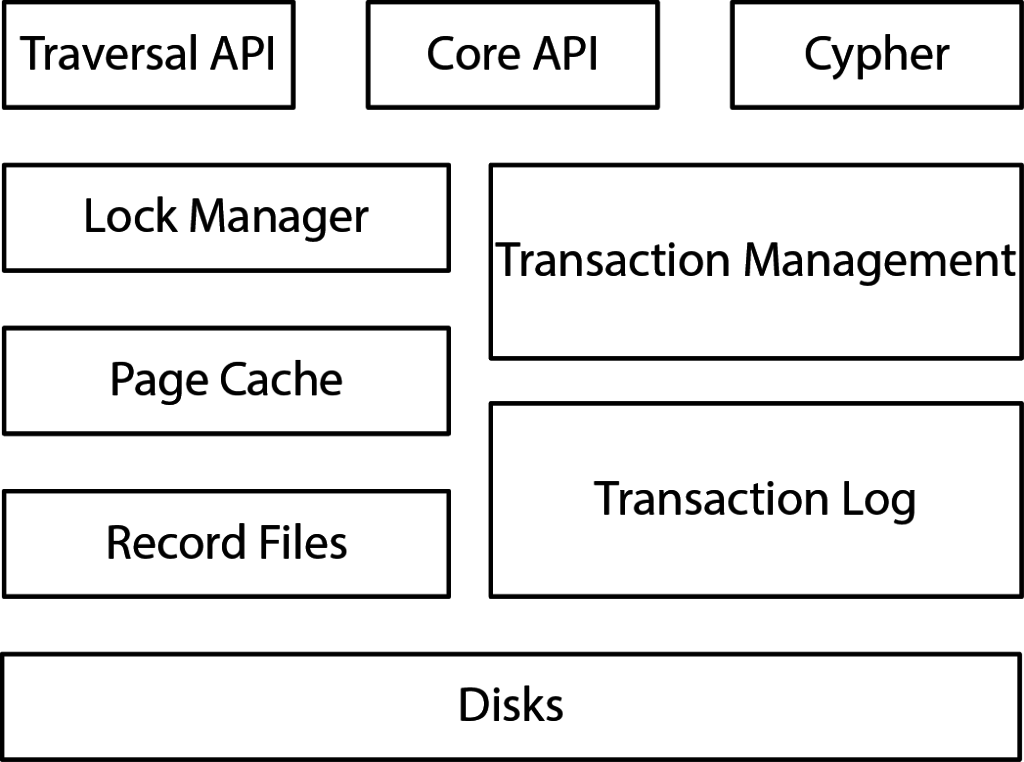
\includegraphics [width=12cm, height=8cm]{Figures/architecture}
	\caption[Architekur von Neo4j]{ aus https://dzone.com/articles/graph-databases-for-beginners-native-vs-non-native(26.08.19)}
	\label{fig:Architecure}
\end{figure}

\subsection{Cypher und APIs für Neo4j}
Im Folgenden werden die Möglichkeiten zum Programmieren mit Neo4j beschrieben. Da es über die Neo4j Treiber möglich ist, Neo4j in mehreren Programmiersprachen zu nutzen und die Anzahl der unterstützten Sprachen stetig steigt, werden im folgenden nur die Kernfunktionen in Java beschrieben und verwendet. Durch die Einbindung einer Erweiterung  ist der Gebrauch der Anfragesprache $GraphQL$ möglich, welche in dieser Evaluation nicht betrachtet wurde.

\subsubsection{Cypher}
Im Gegensatz zu den relationalen Datenbanken gibt es bei Graphdatenbanken keine standardisierte Anfragesprache, welche in den meisten Graphdatenbanken Verwendung findet \parencite{han2011survey}. In Neo4j besteht seit dem Jahr 2000 die Möglichkeit, die deklarative Anfragesprache $Cypher$ zu verwendenden  \parencite{francis2018cypher}. Cypher wird von Neo4j Inc. entwickelt und wurde ursprünglich ausschließlich für die Neo4j Datenbank verwendet. Seit Oktober 2015  findet Cypher als $openCypher$ Gebrauch in anderen Systemen \parencite{francis2018cypher}. Für die APIs von Neo4j sind Kenntnisse in der Programmiersprache Java bzw. einer durch die Neo4j-Treiber unterstützten Programmiersprachen notwendig. Cypher bildet eine Möglichkeit ohne diese Kenntnisse die  Datenbank anzusteuern \parencite{vukotic2015neo4j}. Die Syntax ist an SQL orientiert. In Cypher wird ein Muster durch den Nutzer angegeben und alle Objekte, die dieses Muster erfüllen, werden zurückgegeben. Die wichtigsten  Prädikate sind: \newline
\textbf{Where}: Wie in SQL werden Objekte hierbei anhand von Attributen gefiltert. \newline
\textbf{Match}: Spezifiziert das Muster in dem Neo4j sucht.
\begin{Verbatim}[frame=single]
MATCH (p1:Person)-[:Friends*2]->(p2:Person) 
WHERE p1.name= ‘Peter’ 
RETURN p2.name
\end{Verbatim}
Hier werden alle Personen-Knoten durchsucht, die mit einer “Friends”-Relation mit dem Personen-Knoten von “Peter” verbunden sind. p1 stellt einen Bezeichner für den Knoten vom Typ “Person” dar, [:Friends] ist eine Relation vom Typ “Friends” und durch “->” wird angegeben, dass es sich um eine ausgehende Kante vom Knoten p1 handelt. Mit der Schreibweise [:Friends*2] wird ausgedrückt, dass es sich um die Tiefe 2 handelt, das heißt es werden Freunde von Freunden gesucht. \newline
\textbf{Return}: Es wird angegeben, welche Objekte bzw. welche Attribute der Objekte, die das Muster erfüllen zurückgegeben werden sollen.\newline
\textbf{Delete}: Wie in SQL  wird ein  oder mehrere Objekte aus der Datenbank entfernt.
\begin{Verbatim}[frame=single]
DELETE (p:Person{name: ‘Peter’})  
\end{Verbatim}
\textbf{With}: Dadurch lassen sich in einer Anfrage Objekte manipulieren bevor sie zu einer weiteren Anfrage gegeben werden. 
\begin{Verbatim}[frame=single]
MATCH (p:Person{name: ‘Peter’})  
WITH COUNT(p) as count  
RETURN count
\end{Verbatim} 
\textbf{Create}: Erzeugt ein Objekt in der Datenbank. 
\begin{Verbatim}[frame=single]
Create (p:Person)
\end{Verbatim}
Hier wird ein Knoten vom Typ Person erzeugt. Es ist auch möglich, mehrere Knoten mit den dazugehörigen Relationen zu erzeugen. Indizes  für die Objekte oder Attribute von Objekten können ebenfalls über Create erzeugt werden.\newline
\textbf{Limit}: Beschränkt die Anzahl, welche durch das Return-Statement zurückgegeben wird 
\begin{Verbatim}[frame=single]
MATCH (p:person) RETURN p.name LIMIT 10
\end{Verbatim} 
Hier werden nur die Namen  von 10 Personen zurückgegeben\newline
\textbf{SUM/COUNT/AVG}: Wie in SQL wird die Summe, die Anzahl oder der Durchschnitt von einer gegebenen Menge gebildet. Solch eine Funktionen ist wird Aggregations-Funktion bezeichnet. \newline \newline
Durch die gegebenen Prädikate beeinflusst der Nutzer so welche Daten mittels des Musters gesucht und zurückgegeben werden. Es besteht keine Möglichkeit, die Art der Berechnung zu beeinflussen. Cypher wird dadurch als nutzerfreundlichere aber auch weniger performante Alternative zu den direkten APIs empfohlen \parencite{vukotic2015neo4j}. In den folgenden Experimenten wurde sowohl Cypher als auch die Core API für einen direkten Vergleich verwendet. Cypher wird in Neo4j ausschließlich auf einem Prozessorkern ausgeführt. Durch das Einbinden von User Defined Functions(UDF) für Cypher ist das Ausführen auf mehreren Prozessorkernen in einigen Fällen möglich. Diese UDFs können von den Nutzer erstellt und zur Verfügung gestellt werden und  durch Bibliotheken wie die Awesome Procedures on Cypher(APOC) verbreitet werden \parencite{APOC}.

\subsubsection{Java Core API}
Als nahe Schnittstelle zu den Kernfunktionen von Neo4j bietet die Java Core API die meisten Kontrolle und besitzt bei richtigem Gebrauch die schnellste Laufzeit \parencite{vukotic2015neo4j}. Zur Verwendung dieser imperativen API sind weitreichende Programmierkenntnisse und Wissen über die Neo4j-Bibliotheken, sowie ein genaues Verständnis  über die Daten in dem Graph erforderlich. Wenn diese Kenntnisse gegeben sind, ist die API flexible verwendbar  und der Nutzer hat einen hohen Einfluss darauf, wie die Anfragen bearbeitet werden sollen und kann eine optimale Berechnungsstrategie angeben \parencite{vukotic2015neo4j}. Gegeben seien folgende Transaktionen: \newline
\begin{Verbatim}[frame=single]
try ( Transaction tx = graphDb.beginTx() )
{
	Node Peter = graphDb.getNodeById(Peter_ID);
	Set<Node> friends = new HashSet<Node>();
	for (Relationship R : Peter.getRelationships(FRIEND)) {  
	  Node friend = R.getOtherNode(userJohn);
	  friends.add(friend);                        
	}
	for (Node friend : friends) {
	  logger.info("Found friend: " + friend.getProperty("name")); 
	}
}

try ( Transaction tx = graphDb.beginTx() )
{
	try ( ResourceIterator<Node> users =
	graphDb.findNodes( labelPerson, "name", "Peter" ) )
	{
	  ArrayList<Node> userNodes = new ArrayList<>();
	  while ( users.hasNext() ){
		userNodes.add( users.next() );
	  }
	  for ( Node node : userNodes ){
		System.out.println("The attribute of user " 
		+ Peter + " is " 
		+ node.getProperty( "attribute" ));
	  }
	}
}
\end{Verbatim}

\noindent In der ersten Transaktion werden alle Freunde von Peter gefunden und zurückgegeben. Die zweite Transaktion gibt die Eigenschaft $attribute$ von  Peter zurück. Der Nutzer gibt jede Transaktion explizit an, so ist es dem System möglich die Transaktionen zu parallelisieren und nicht ausgelastete Prozessorkerne zu nutzen.

\subsubsection{Traversal API}
Die deklarative Travesal API dient zum spezifizieren von Traversierungen im Graph, sie ist näher an den Kernfunktionen von Neo4j als Cypher und weiter entfernt als die Core API. Die Traversal API erlaubt einen Zugriff auf Neo4j, welcher  abstrakter als die Core API ist. Der Nutzer muss keine genaues Verständnis von den Daten im Graphen haben. Es wird eine Beschreibung angegeben, wie eine Traversierung  ausgeübt werden soll und diese wird auf einen Graphen anwenden. Gegeben seine folgende Traversierungen:
\begin{Verbatim}[frame=single]
private Traverser getFriends(final Node person)
{
	TraversalDescription td = graphDb.traversalDescription()
		.depthFirst()
		.relationships( RelTypes.FRIEND, OUTGOING )
		.evaluator( Evaluators.toDepth(2) );
	return td.traverse( person );
}

private Traverser getEverytingBreathFirst(final Node person)
{
	TraversalDescription td = graphDb.traversalDescription()
		.relationships(RelTypes.RELATIONSHIP3 )
		.breadthFirst();
	return td.traverse( person );
}
\end{Verbatim}
Zusammengefasst wäre die erste Traversierung: Suche alle Verbindungen von dem Anfangsknoten über die Relation FRIEND bis zur Tiefe 2. Die zweite Traversierung geht über den gesamten Graphen, bis alle Knoten einmal erreicht werden. Beim Traversieren kann der  Nutzer zwischen 3 grundsätzlichen Vorgehen wählen: Breitensuche, Tiefensuche und bidirektionale Traversierung, diese haben abhängig von der Struktur des Graphen und der gestellten Anfrage eine unterschiedliche Laufzeit \parencite{vukotic2015neo4j}. In  Abbildung \ref{fig:Search} werden durch die blauen Linien die Reihenfolgen der beiden Suchalgorithmen dargestellt. \newline
\textbf {Breadth-First-Search(Breiten-Suche)} : Zuerst werden alle Knoten mit derselben Distanz betrachtet, danach werden alle Knoten mit der nächst höheren Distanz betrachtet, dies wird solange ausgeübt bis alle Knoten betrachtet wurden. \newline
\textbf {Depth-First-Search(Tiefen-Suche)}: Zunächst wird ein Knoten der Tiefe 1 gewählt, ausgehend von diesem Knoten wird ein nächsttieferer Knoten, der noch nicht betrachtet wurden, gewählt. Dies wird so lange wiederholt bis keine neuen nächsttieferen Knoten hinzugefügt werden können, danach so lange rückwärts gegangen bis ein Knoten zu erreichen ist, der noch nicht betrachtet wurde. \newline
\textbf {Bidirektionale Traversierung}: Es werden 2 Knoten gewählt und von jedem Knoten wird eine Traversierung  mit Tiefen- oder Breitensuche gestartet, die beiden Traversierungen müssen nicht über die gleichen Relationen verlaufen oder im selben Schrittintervall vollzogen werden. Bei dem Treffen der beiden Traversierungs-Pfade wird von dem Nutzer ein Verhalten definiert.
\FloatBarrier
\begin{figure}[!htb]
	\centering
	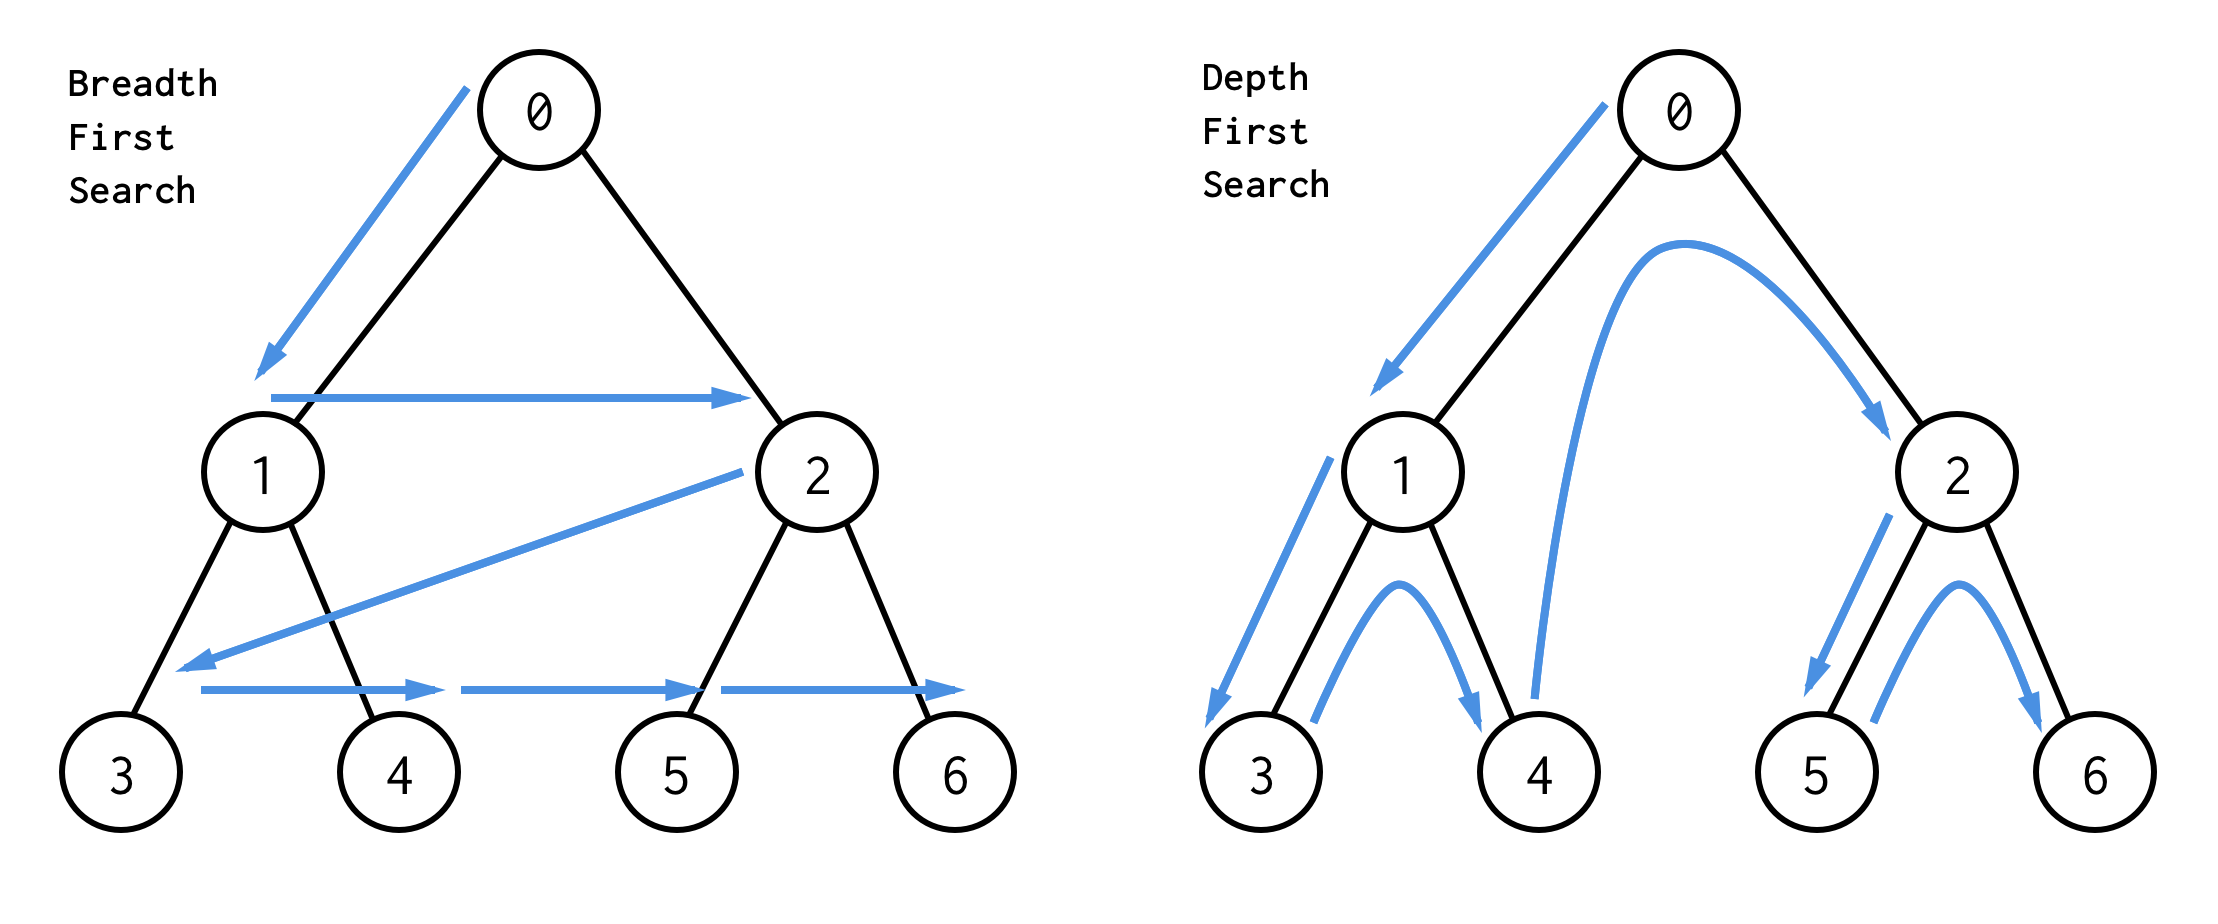
\includegraphics [width=14cm, height=6cm]{Figures/search}
	\caption[Breiten- und Tiefensuche]{ aus http://mishadoff.com/blog/dfs-on-binary-tree-array/.}
	\label{fig:Search}
\end{figure} 
\FloatBarrier
\noindent Wenn der Nutzer mit der Struktur der Daten in dem Graph vertraut ist, kann die ausgewählte Methode eine erheblichen Performanzunterschied  hervorbringen \parencite{vukotic2015neo4j}. 

\subsection{Anfragebearbeitung und Planoptimierung}
Nach Angaben von Neo4j werden Anfragen in Cypher, nach folgendem Muster bearbeitet \parencite{Optimizer}:
\begin{enumerate}
	\item Umwandeln der Eingabe in einen abstrakten Syntax Baum (ASB)
	\item Optimieren des ASB
	\item Erstellen eines Anfragegraphen aus dem Baum
	\item Erstellen eines logischen Plans
	\item Optimieren des logischen Plan 
	\item Erstellen eines Ausführungsplan aus dem logischen Plan
	\item Ausführen die Anfrage mit Hilfe des Ausführungsplans  
\end{enumerate}
Die Schritte 2-5 werden vom Cypher Query Optimizer übernommen. \newline \newline
1. Die Eingabe wird auf semantische Fehler bei den Typen und auf allgemeine syntaktische Fehler überprüfst. Wenn keine Fehler erkannt wurde, wird die Eingabe in einen ASB umgewandelt, welcher die Semantik der Eingabe darstellt. \newline
\newline
2. Die Optimierung des ASB beinhaltet folgende Schritte: 
\begin{enumerate}[label=(\roman*)]
	\item Alle Labels, die sich in einem \textbf{Match} befinden, werden in das \textbf{Where}-Prädikat verschoben
	\item  Semantisch-äquivalente \textbf{Where}-Prädikate werden zusammengefasst
	\item Ersetze alle Synonyme zum wie: \textbf{RETURN * => RETURN x as x, y as y}
	\item Fasse Konstanten zusammen zum wie: \textbf{3 + 3 => 6}
	\item Setze bei anonymen Knoten einen Namen ein zum wie: \textbf{ MATCH () => MATCH (n:Person)}
	\item Ersetze das Gleichheitszeichen durch ein 'IN'wie: \textbf{MATCH (n) WHERE id(n) = 12 => MATCH n WHERE id(n) IN [12]}
\end{enumerate}
3. Durch das Erstellen eines Anfragegraphen wird ein abstraktere Darstellung für die Anfrage erzeugt.\newline \newline
4. Aus dem Anfragegraphen wird ein logischer Plane für jede Anfrage erzeugt. Dieser Plan ist ein Baum mit maximal 2 Kindern, welche die verwendeten Operatoren darstellen. Dies gleicht einem logischen Plan für relationale Datenbanken. Aus dem logische Plan wird der geschätzte Bearbeitungsaufwand für eine Anfrage gelesen. Der Aufwand wird aus den benötigten I/O-Operatoren auf den Speicher oder Indizies und den durchzuführenden Traversierungen ermittelt. Bei jedem Durchgang werden mehrere Pläne für eine Anfrage erzeugt, der Optimierer wählt aus diesen Plänen mit einem gierigen Suchalgorithmus einen Plan aus, welcher nahe am optimalste Plan ist, aber garantiert nicht der langsamste Plan ist. \newline \newline
5. Nachdem die Pläne erstellt wurden und einer dieser Pläne ausgewählt wurde, wird der ausgewählte Plan nochmals optimiert. Das heißt alle Komponenten werden so weit wie möglich vereinfacht und Redundanzen werden zusammengeführt. Jede Art von Verschachtelung, wie ein Match-Prädikat in einer Where Bedingung wird aufgelöst. Die Arbeit des Optimierers ist mit dem 5. Schritt abgeschlossen \newline \newline
6. Der logische Plan gibt vor, wie die Anfrage semantisch bearbeitet werden soll, es wird nicht spezifiziert mit welchen Mitteln die Anfrage ausgeführt werden soll. Der Ausführungsplan baut auf dem logischen Plan auf und gibt für die benötigten Operatoren eine hierarchische Anordnung von physischen  Implementierungen vor. Dieser Plan wird durch die Database Engine erstellt.  \newline \newline
7. Die Operatoren in dem Ausführungsplan werden während der Laufzeit in der vorgegebenen Reihenfolge ausgeführt. 


\subsection{Speicherverwaltung in Neo4j}
Graphdatenbanken besitzen eine andere Speicherverwaltung als relationale Datenbanken \parencite{angles2012comparison}. In Neo4j wird der Speicher in sogenannten Record Files unterteilt. Diese Dateien speichern jeweils einen Teil des Graphen wie Knoten, Kanten, Attribute etc. ab. Die Objekte besitzen in den Dateien eine feste Größe, dies erlaubt einen Zugriff in konstanter Zeit \parencite{robinson2013graph}. Wenn der Knoten mit der ID 100 gesucht wird und ein einzelner Knoten X Bytes groß ist, wird der gesuchte Knoten bei Byte 100*X beginnen. Die genaue Größe  variiert, je nach betrachteter Neo4j Version, seit Neo4j Version 3 besitzt ein Knoten die Größe 15 Byte und werden in der Datei node-store gespeichert \parencite{Storage}. Nach \parencite{robinson2013graph} werden die Objekte wie folgt verwaltet:
\subsubsection{Verwaltung der Knoten im Speicher}
Ein Knoten im Knotenspeicher wird folgendermaßen dargestellt: Das erste Byte kennzeichnet, ob der Knoten verwendet wird bzw. genutzt werden kann. Die nachfolgenden 4 Bytes kennzeichnen die ID für die erste Relation, die mit dem Knoten verbunden ist. Die darauffolgenden 4 Bytes beschreiben das erste Attribute des Knoten. Die nächsten 5 Bytes verweisen auf ein Label, welches gegebenenfalls verwendet wurde und sich im Label-Store befindet. Das letzte Byte ist für bestimmte Flags und für zukünftige Verwendungszwecke. 
\subsubsection{Verwaltung der Kanten im Speicher}
Die Kanten werden in dem Relationsspeicher gespeichert. Jeder Eintrag besitzt die IDs zu den zugehörigen Knoten, einen Zeiger zu dem Relationstypen, welcher in dem Relationstypspeicher gespeichert ist, der Zeiger zu den vorherigen und nächsten Relationen von den beiden zugehörigen Knoten und ein Flag, das angibt ob die betrachtete Relation die erste in einer Liste von zugehörigen Relationen im Graphen ist. 
\subsubsection{Verwaltung der Attribute im Speicher}
Neo4j wird als property graph database bezeichnet, dort kann jeder Knoten und jede Kante Attribute besitzen. Die Attribute befinden sich im Attributsspeicher. Jeder Eintrag zu einem Attribut ist in 1-4 Blöcke und einer ID zu einem nächstfolgenden Attribut unterteilt. Jeder der Blöcke beinhaltet Informationen über einen Typen, welcher ein String, ein Array oder ein Java-Standard Typ sein kann und einen Zeiger auf ein Index zu dem Namen des Attributs.  
\subsubsection{Indizies}
Ein Index ist eine redundante Kopie von Daten in einer Datenbank, es kann auf ein Element direkt zugegriffen werden, ohne dass über die gesamte Datenstruktur iteriert werden muss. Dadurch wird die Suche nach diesen Daten beschleunigt.Neo4j besitzt die Index-freie Nachbarschafts Eigenschaft, dadurch sind die Knoten nicht über einen Index  sondern, direkt über Relationen verbunden. Bei einer GDB ohne diese Eigenschaft werden die Knoten durch einen globalen Index verbunden und eine weitere Datenstruktur wie zum wie ein Binärbaum oder eine Hash-Tabelle wird für das Traversieren verwendet \parencite{robinson2013graph}. \newline
Neo4j nutzt Indizes ausschließlich für Attribute und erlaubt das Erstellen eines Index zu einem oder mehreren Attributen. Sobald ein Index zu einem angegebenen Attribute erstellt wurde, wird dieser immer aktuell gehalten \parencite{Index}.  	
\subsubsection {Traversierung im Speicher}
Die festgelegte Größe der Knoten und Kanten hat als Ziel, die Traversierung zu beschleunigen \parencite{robinson2013graph}. Eine einfache Traversierung wird beschrieben wie folgt: 
\begin{enumerate}
	\item Starten bei einem Eintrag in den Knotenspeicher
	\item Lesen des gegebene Byte für die ID zur ersten Relation und betrachten des entsprechenden Eintrags im Relationsspeicher mit dieser ID
	\item Ausgehend von dem Eintrag im Relationsspeicher wird der Zeiger zum dazugehörigen Knoten aufgerufen.
	\item Springen zu der Knoten im Knotenspeicher
\end{enumerate}
Diese Traversierung beschreibt das Suchen eines benachbarten Knotens.
\subsubsection{Caching im Speicher}
Neoj4 nutzt den LRU-K page-affined cache, wodurch die Datenbank aufgeteilt wird und eine feste Anzahl von Teilen wird im Hauptspeicher gehalten. Die Auswahl der Teile, die im Speicher gehalten werden, geschieht nach dem least frequently used(LFU) Vorgehen. Diese Methode besagt, dass ein Teil, der selten benutzt wird, aus dem Speicher entfernt wird und ein häufig genutzter Teil im Speicher gehalten wird\parencite{robinson2013graph}.
\subsection{CAP und ACID unter Neo4j}
Das CAP-Theorem charakterisiert das Verhalten einer Datenbank anhand von folgenden 3 Eigenschaften: Consistency(Konsistenz), Availability(Verfügbarkeit), Partitionstoleranz \parencite{simon2000brewer}. Konsistenz beschreibt die Eigenschaft, dass die Daten in allen Partitionen zur selben Zeit dieselben Werte besitzen und das gleiche Verhalten aufweisen. Verfügbarkeit beschreibt die Möglichkeit, zu jeder Zeit eine Anfrage an das System stellen zu können und auch zu jeder Zeit eine Antwort auf die gestellte Anfragen bekommen zu können. Partitionstoleranz gewährleistet, dass sich das Verhalten des Systems nicht verändert, wenn das System in mehrere kleinere Teilstück, auch  Partitionen genannt, zerteilt wird. Alle Partitionen müssen das gleiche Verhalten wie das gesamt System aufweisen \parencite{simon2000brewer}. Neo4j erfüllt die Bedingung der Verfügbarkeit und der  Partitionstoleranz \parencite{vukotic2015neo4j} und wird so als “AP-Database” bezeichnet. \newline
Die ACID Eigenschaft setzt sich aus 4 Eigenschaften zusammen, die das Verhalten der Transaktionen einer  Datenbank beschreiben \parencite{haerder1983principles}. Atomicity(atomisch) beschreibt, dass jede Transaktion einzeln betrachtet wird und entweder komplett fehlschlagen oder komplett erfolgreich sein kann. Durch Consistency(consistenz) kann jede Transaktion nur valide Daten verwenden und den validen Zustand einer Datenbank nicht in einen nicht-validen Zustand überführen. Isolation erwartet, dass jede Transaktion unabhängig von einer parallel-laufenden Transaktion abläuft und keine dieser Transaktionen beeinflusst. Durability(haltbarkeit) ist gegeben, wenn der Effekt einer Transaktion auf den Speicher ausgeübt wurde und auch bei einem Absturz des Systems bestehen bleibt \parencite{haerder1983principles}. \newline Solange Neo4j auf einem einzelnen System läuft und nicht das High Availability Feature der Enterprise Edition nutzt, ist es ACID konform \parencite{holzschuher2013performance}. Das atomische und haltbare Verhalten wird durch das sogenannte write-ahead log versichert. Bei diesem Mechanismus  werden alle Operationen einer Transaktionen nach dem Beenden der Transaktion in einem Log-File  festgehalten, bevor diese  den Speicher beeinflussen, so kann auch bei einem Absturz des Systems das Log-File genutzt werden um ein vorherige Transaktion zu wiederholen.  Dieses Log-File wird auch für die High-Availability  genutzt, welche es erlaubt, die Datenbank in einem Netzwerk auf mehrere Systeme zu verwenden, dennoch ist es nicht mehr möglich, ein  ACID Verhalten zu gewährleisten, da keine absolute Garantie für ein  atomisches und konsistente Verhalten gibt \parencite{vukotic2015neo4j}. Eine weitere Eigenschaft für das isolierte Verhalten bildet das Verhindern von Deadlocks innerhalb der Transaktion. Zur Verhinderung von Deadlocks wird “RWLock” verwendet, was eine Implementierung des Java “ReentrantReadWriteLock” für Neo4j ist. Dieser verwaltet alle Schreibsperren, die während einer Transaktion erstellt werden und versucht, potentielle Deadlocks zu erkennen \parencite{raj2015neo4j}.
\section {Modi zur Bedienung von Neo4j}
Wenn der Nutzer Neo4j nicht über die Anwendungen $Neo4j Browser/Desktop$ sondern über ein Programmiersprache nutzen möchte,  lässt sich Neo4j in 2 Modi nutzen, den eingebetteten Modus und den Server Modus. Diese Modi geben an wie die Bibliotheken von Neo4j, welche für die Anfragen des Nutzer benötigt werden, aufgerufen und verwendet werden. Dafür wird das Verhalten der Java Virtual Machine (JVM), welche die Kompatibilität des geschriebenen Java-Codes gewährleistet, angepasst. Der verwendete Speicher ist für beide Modi derselbe.

\subsection{Der eingebettete Modus}
Der eingebettete Modus erlaubt es dem Nutzer die  Bibliotheken von Neo4j mittels jeder Programmiersprache, die von der JVM unterstützt wird und für die ein Treiber zur Verfügung steht, zu nutzen und so Anfragen an die Datenbank zu stellen. Alle Bibliotheken von Neo4j werden durch den GraphDataBaseService von Neo4j verwaltet. Der Eingebettete Modus wird für die meisten Anwendungen, die auf einem einzelnen System laufen, empfohlen \parencite{raj2015neo4j}. Dies ist dadurch begründet, dass das Gesamtsystem im einbetteten Modus schneller läuft als im Server Modus, aber auch nur auf einem System genutzt werden kann, da sowohl alle Neo4j Funktionen als auch die Anfragen in der selben JVM agieren. Der Nutzer hat so volle und alleinige Kontrolle über jede Transaktion und kann jede zur Verfügung stehenden Funktion der API nutzen. Daraus resultiert, dass er Nutzer für ein sicheres Starten und Beenden der Datenbank in seiner Sitzung verantwortlich ist \parencite{robinson2013graph}.  Verdeutlicht wird diese Struktur in Abbildung \ref{fig:Embedded}.
\begin{figure}[!htb]
	\centering	
	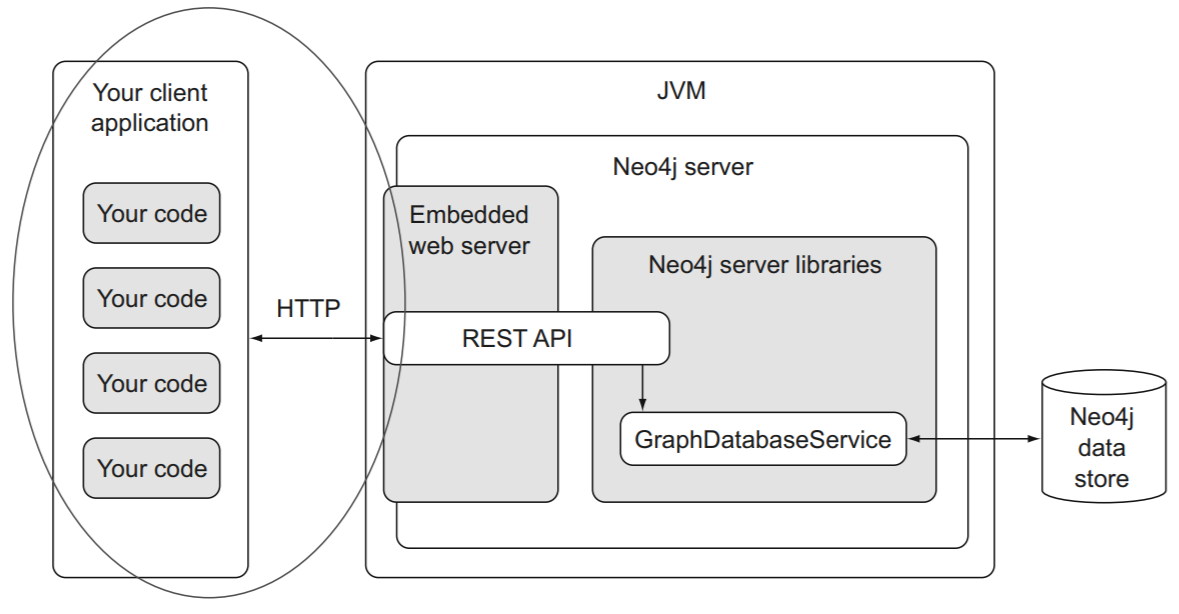
\includegraphics [width=10cm, height=5cm]{Figures/embedded}
	\caption[Eingebetteter Modus]{aus https://livebook.manning.com/book/neo4j-in-action/chapter-10/9 (16.07.19)}
	\label{fig:Embedded}
\end{figure}

\subsection{Der Server Modus} \label{Server}
Im Server Modus werden alle Anfragen von den Nutzern in einem eigenen Prozess verwaltet und mittels HTTP(Hypertext Transfer Protocol) als JSON-Formatiertes Dokument an die sogenannte REST API übermittelt \parencite{robinson2013graph}. Die REST API läuft in der Neo4j JVM und  verwaltet alle eintreffenden Anfragen der Nutzer und gibt diese an den GraphDatabaseService weiter, welcher die von Neo4j zur Verfügung gestellten Funktionen verwaltet. \newline 
Der Server Modus ist für die Verwendung der High-Availability Fuktion empfohlen, welche das Nutzen der Datenbank auf mehren Systemen erlaubt.\parencite{raj2015neo4j}. Da die Anfragen des Nutzer getrennt von der Neo4j JVM verwaltet werden und so mehrere Nutzer die Möglichkeit besitzen, diese Funktionen zu Nutzen. Durch die  Übertragungsverzögerung innerhalb der Netzwerks und dem Übertragen durch eine weitere API ist die Verzögerung höher als die des eingebetteten Modus. Dieser Modus wird in Abbildung \ref{fig:Server} verdeutlicht.
\begin{figure}[!htb]
	\centering
	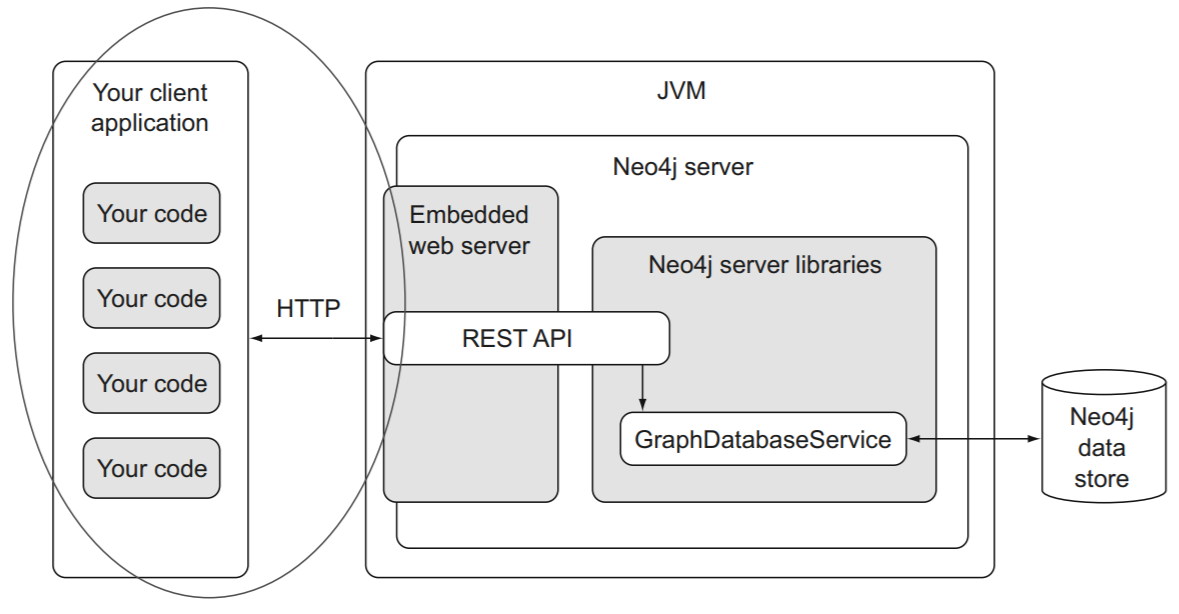
\includegraphics [width=10cm, height=5cm]{Figures/server}
	\caption[Server Modus]{aus https://livebook.manning.com/book/neo4j-in-action/chapter-10/9 (16.07.19)}
	\label{fig:Server}
\end{figure}

